\documentclass[usenames,dvipsnames,notes,11pt,aspectratio=169]{beamer}
\usepackage{ifthen}
\usepackage{xcolor}
\usepackage{pgfplots}
\usepackage{amsmath}
\usepackage{centernot}
\usepackage{pifont}
\usepackage{tabularx}
\usepackage{makecell}
\usepackage{cuted}
\usepackage{booktabs}
\usepackage{array}
\usepackage{setspace}
\usepackage{CJKutf8}
\usepackage{textcomp}


%\usepackage{pgfpages}
%\setbeameroption{show notes on second screen}

\pgfplotsset{compat=1.17,
    every axis/.append style={
            font=\large,
            line width=1pt,
            tick style={line width=0.8pt}}}

\input ../beamer-style
\input ../std-macros
\input ../macros

\AtBeginSection[]
{
    \begin{frame}
        \frametitle{Table of Contents}
        \tableofcontents[currentsection]
    \end{frame}
}



\title[CSCI-GA.2590]{Machine Learning Basics}
\author[He He]{He He
}
\institute[NYU]{
    
\includegraphics[height=1cm]{../figures/nyu-logo}\\
}
\date{January 24, 2023}

\begin{document}

\begin{frame}
\titlepage
\end{frame}

\section{Generalization}

\begin{frame}
    {Rule-based approach}
\begin{figure}
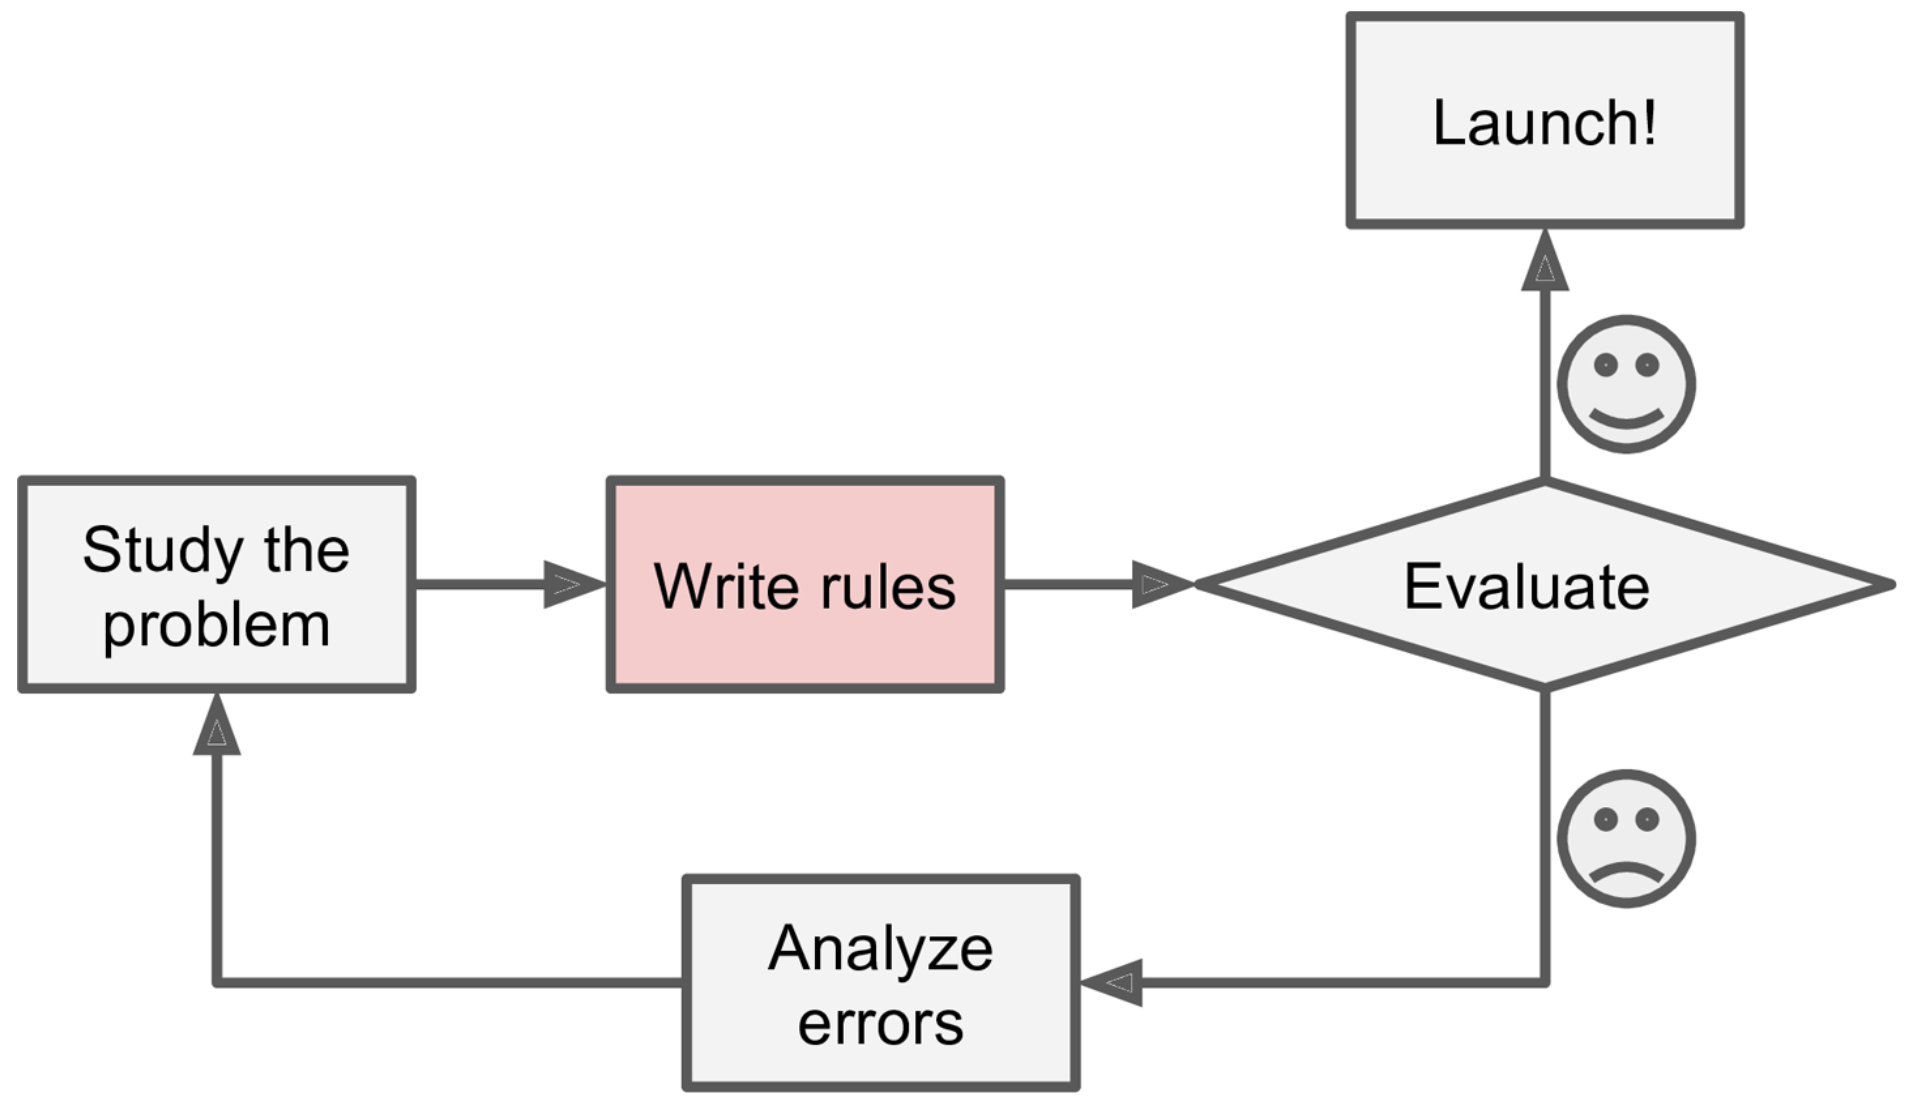
\includegraphics[height=0.7\textheight]{figures/geron-fig1-1}
    \caption{{Fig 1-1 from \emph{Hands-On Machine Learning with Scikit-Learn and TensorFlow} by Aurelien Geron (2017).}}
\end{figure}
\end{frame}

\begin{frame}
    {Machine learning approach}
\begin{figure}
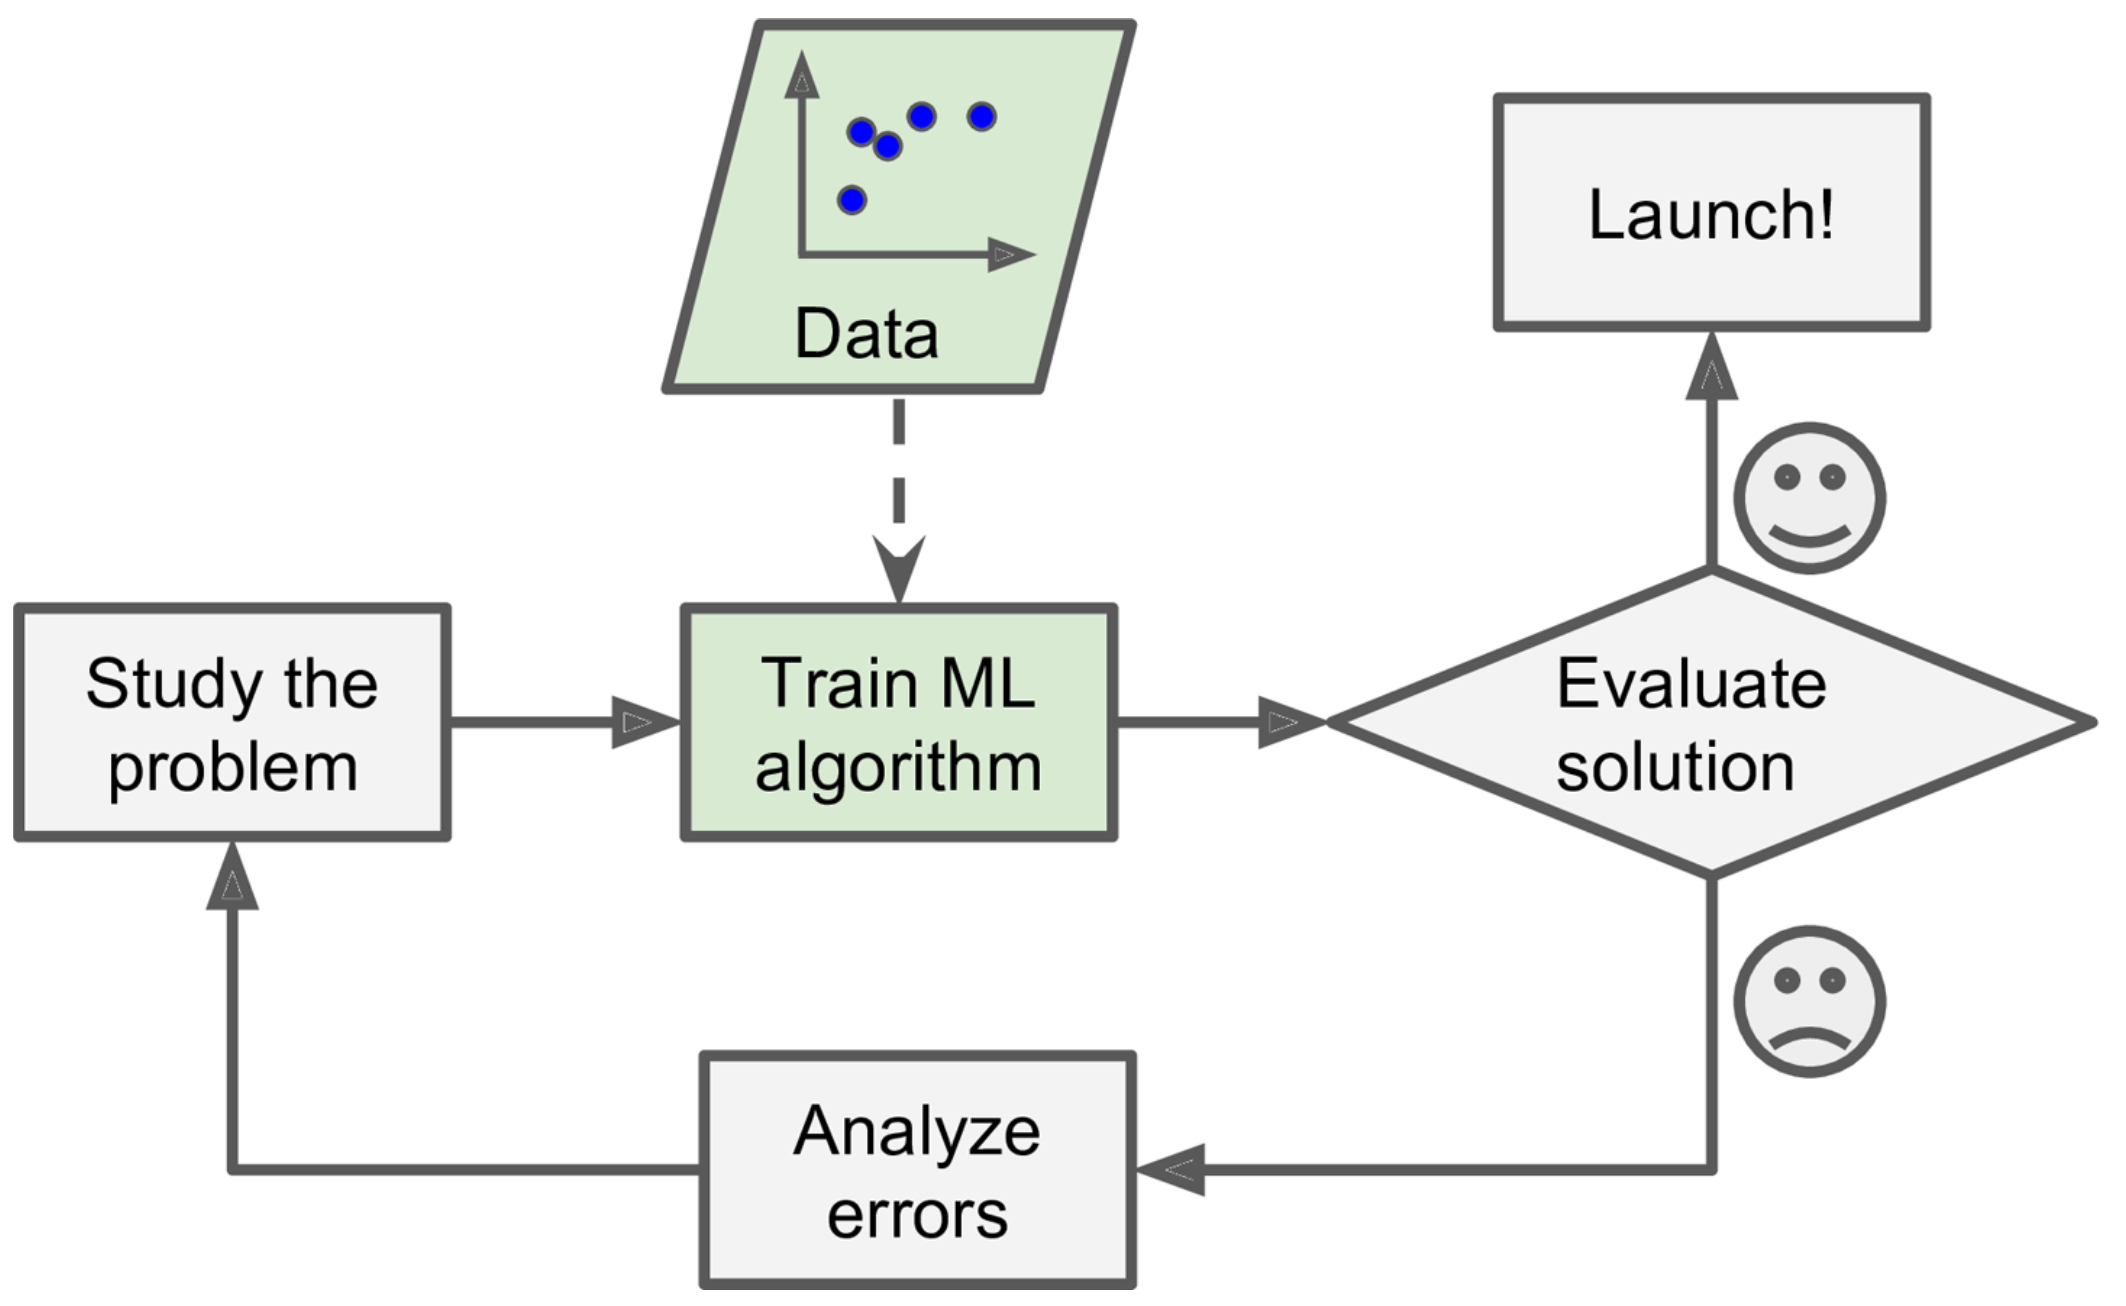
\includegraphics[height=0.7\textheight]{figures/geron-fig1-2}
    \caption{{Fig 1-2 from \emph{Hands-On Machine Learning with Scikit-Learn and TensorFlow} by Aurelien Geron (2017).}}
\end{figure}
\end{frame}

\begin{frame}
    {Example: spam filter}
    
    \begin{itemize}
        \itemsep1em
        \item Rules
            \begin{itemize}
                \item[] Contains ``Viagra''
                \item[] Contains ``Rolex''
                \item[] Subject line is all caps
                \item[] ... 
            \end{itemize}
        \item Learning from data
            \begin{enumerate}
                \item Collect emails labeled as spam or non-spam 
                \item Design features, e.g., first word of the subject, nouns in the main text
                \item Learn a binary classifier 
            \end{enumerate}
    \end{itemize}
    \medskip
    \think{Pros and cons of each approach?}
\end{frame}

\begin{frame}
    {Key challenges in machine learning}
    \begin{itemize}
        \itemsep1em
        \item Availability of large amounts of (annotated) data
            \begin{itemize}
                \item Data collection: scraping, crowdsourcing, expert annotation
                \item Quality control: data quality can have large impact on the final model (garbage in garbage out)
                \item Don't take it for granted: always check the data source!
            \end{itemize}
    \end{itemize}
    \think{How would you collect a dataset for the spam filtering task?}
\end{frame}

\begin{frame}
    {Key challenges in machine learning}
    \begin{itemize}
        \item \textbf{Generalize} to unseen samples
            \begin{itemize}
                \item We want to build a model: $h\colon \sX \text{ (input space)} \rightarrow \sY \text{ (output space)}$
                \item It is easy to achieve high accuracy on the training set.
                \item But we want the model to perform well on unseen data, too.
                \item How should we evaluate the model? 
               %\item Given the training set: $m$ samples from $\sD$ $\pc{(x^{(i)}, y^{(i)})}_{i=1}^m$
               % \item Assume that there is a (unknown) data generating distribution: $\sD$ over $\sX\times\sY$
               %\item Goal: \blue{minimize }:$\text{minimize}\quad 
               %    \mathbb{E}_{(x,y)\sim\sD}\pb{\text{error}(h,x,y)}$ (estimated on the test set)
            \end{itemize}
    \end{itemize}
\end{frame}

\begin{frame}
    {Empirical risk minimization (ERM)}

    \begin{itemize}[<+->]
        \item Assume a data generating distribution $\sD$ over $\sX\times\sY$ (e.g., spam writers and non-spam writers)
        \item We have access to a training set: $m$ samples from $\sD$ $\pc{(x^{(i)}, y^{(i)})}_{i=1}^m$
        \item We can measure the goodness of a prediction $h(x)$ by comparing it against the groundtruth $y$ using some \textbf{loss function}
        \item Our goal is to minimize the \blue{expected loss} over $\sD$ (\textbf{risk}):
            $$
\text{minimize}\quad \mathbb{E}_{(x,y)\sim\sD}\pb{\mathrm{error}(h,x,y)} \;,
            $$
            but it \red{cannot be computed} (why?).
\item Instead, we minimize the \blue{average loss on the training set} (\textbf{empirical risk})  %over $\sH$
    $$
    \text{minimize}\quad \frac{1}{m}\sum_{i=1}^m \mathrm{error}(h, x^{(i)}, y^{(i)})
    $$

%\item In the limit of infinite samples, empirical risk converges to risk (LLN).
        \item Key question: does small empirical risk imply small risk? 
    \end{itemize}
\end{frame}

%\begin{frame}
%    {Error decomposition}
%\end{frame}

\begin{frame}
    {Overfitting vs underfitting}
    \begin{itemize}
        \item[] [board]
        \item Trivial solution to (unconstrained) ERM: \red{memorize} the data points
        \item Need to extrapolate information from one part of the input space to unobserved parts!
        \item Solution: constrain the prediction function to a subset, i.e.\ a \textbf{hypothesis space} $h\in \sH$.
            \pause
        \item Trade-off between complexity of $\sH$ and generalization 
        \item Question for us: \blue{how to choose a good $\sH$ for certain domains}
    \end{itemize}
\end{frame}

\begin{frame}
    {Summary}
    \begin{enumerate}
        \itemsep2em
        \item Obtain training data $D_{\text{train}}=\pc{(x^{(i)}, y^{(i)})}_{i=1}^n$.
        \item Choose a loss function $L$ and a hypothesis class $\sH$ (\blue{domain knowledge}).
        \item Learn a predictor by minimizing the empirical risk (\blue{optimization}).
    \end{enumerate}
\end{frame}

\section{Loss functions}

\begin{frame}
    {Setup}
    \begin{itemize}
        \itemsep1em
        \item Task: binary classification $y\in\pc{+1, -1}$
        \item Model: $f_w\colon \sX \rightarrow \bR$ parametrized by $w \in \bR^d$
            \begin{itemize}
                \item Output a score for each example
            \end{itemize}
        \item Prediction: $\text{sign}(f_w(x))$
            \begin{itemize}
                \item Positive scores are mapped to the positive class 
            \end{itemize}
        \item Goal: quantify the goodness of the model output $f_w(x)$ given $y$
    \end{itemize}
\end{frame}

\begin{frame}
    {Zero-one loss}
    
    First idea: check if the prediction is the same as the label

            \begin{align}
                L(x, y, f_w) = \1\pb{\text{sign}(f_w(x)) = y} 
                = \1\pb{\underbrace{yf_w(x)}_{\textstyle\text{margin}}\le 0}
                %= \1\pb{{yf_w(x)} \le 0}
            \end{align}
    \begin{figure}
        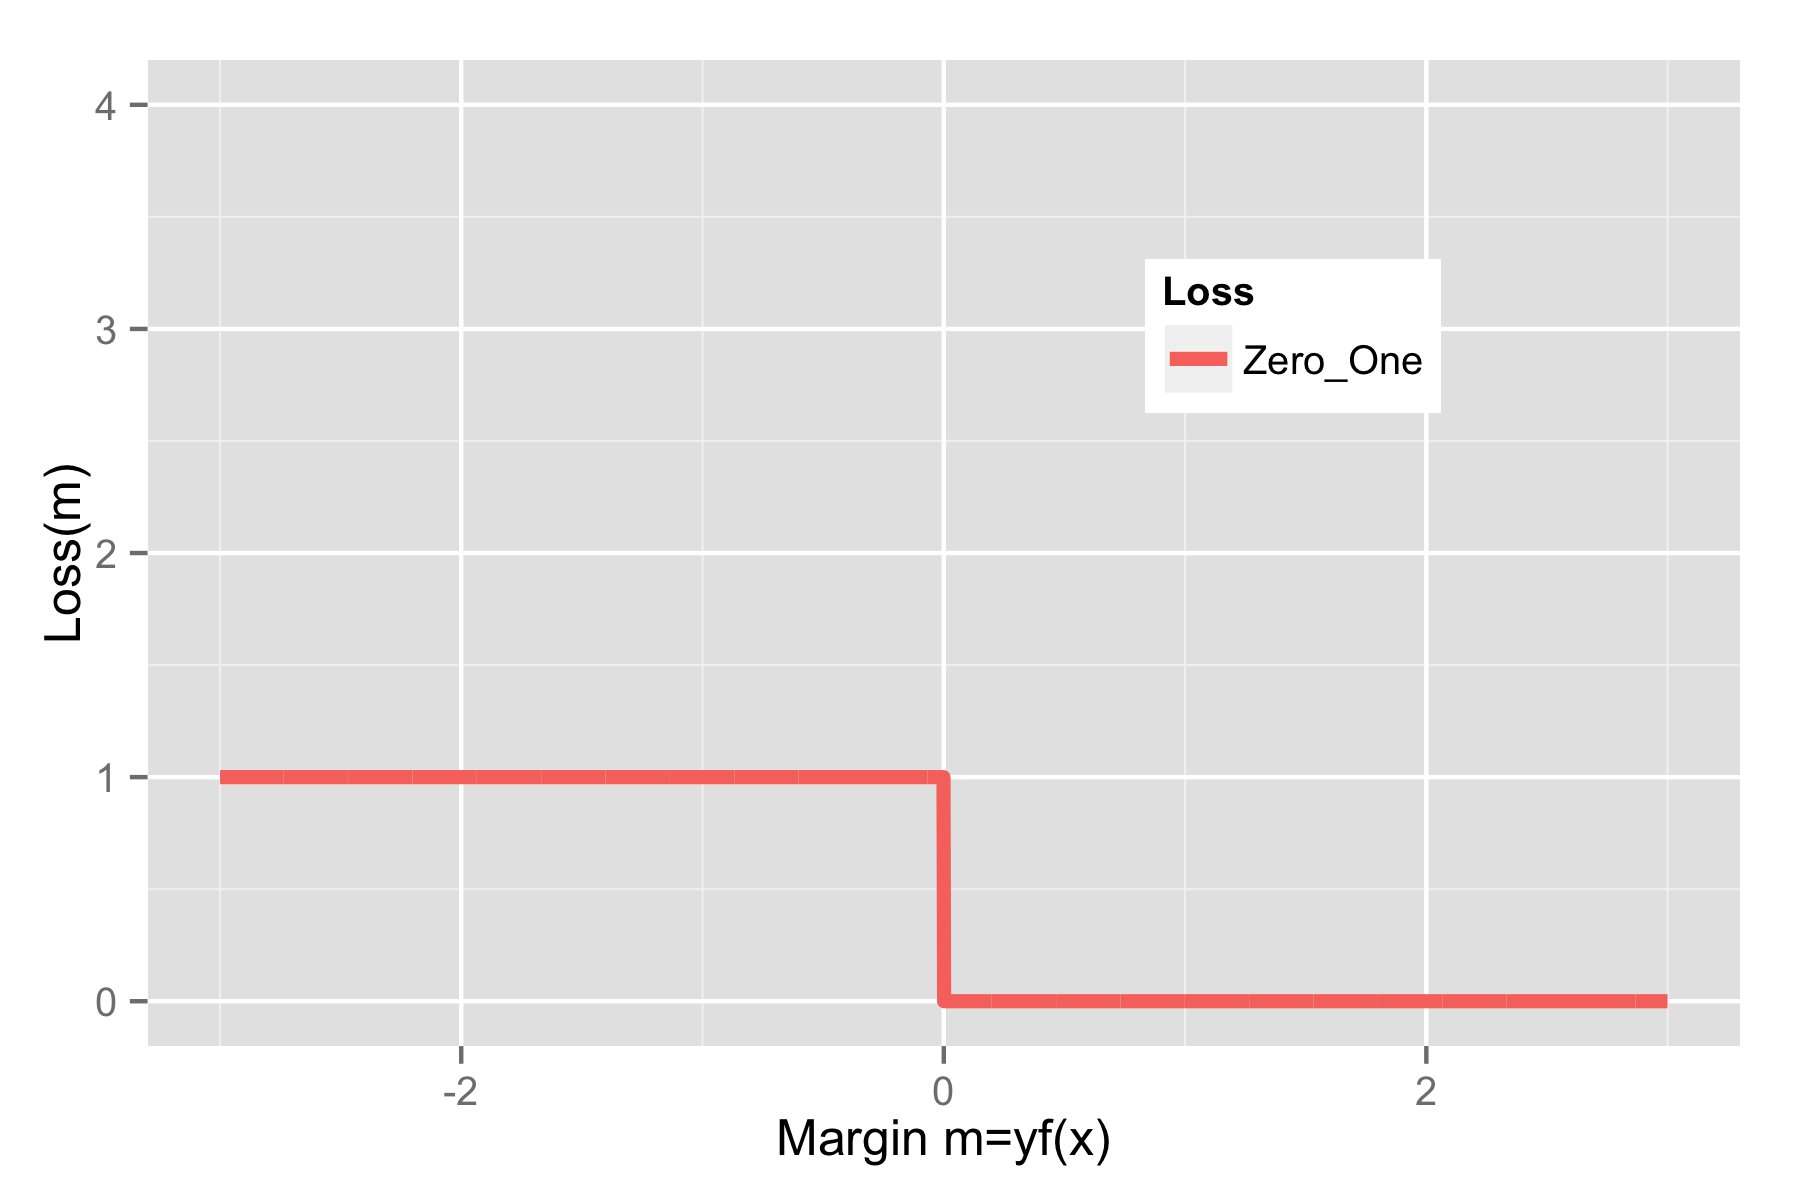
\includegraphics[height=4cm]{figures/loss.Zero_One.png}
    \end{figure}
    \pause
    Problem: \red{not differentiable}
\end{frame}

\begin{frame}
    {Hinge loss}
    $$
    L(x,y,f_w) = \max(1-yf_w(x), 0)
    $$
    \begin{figure}
        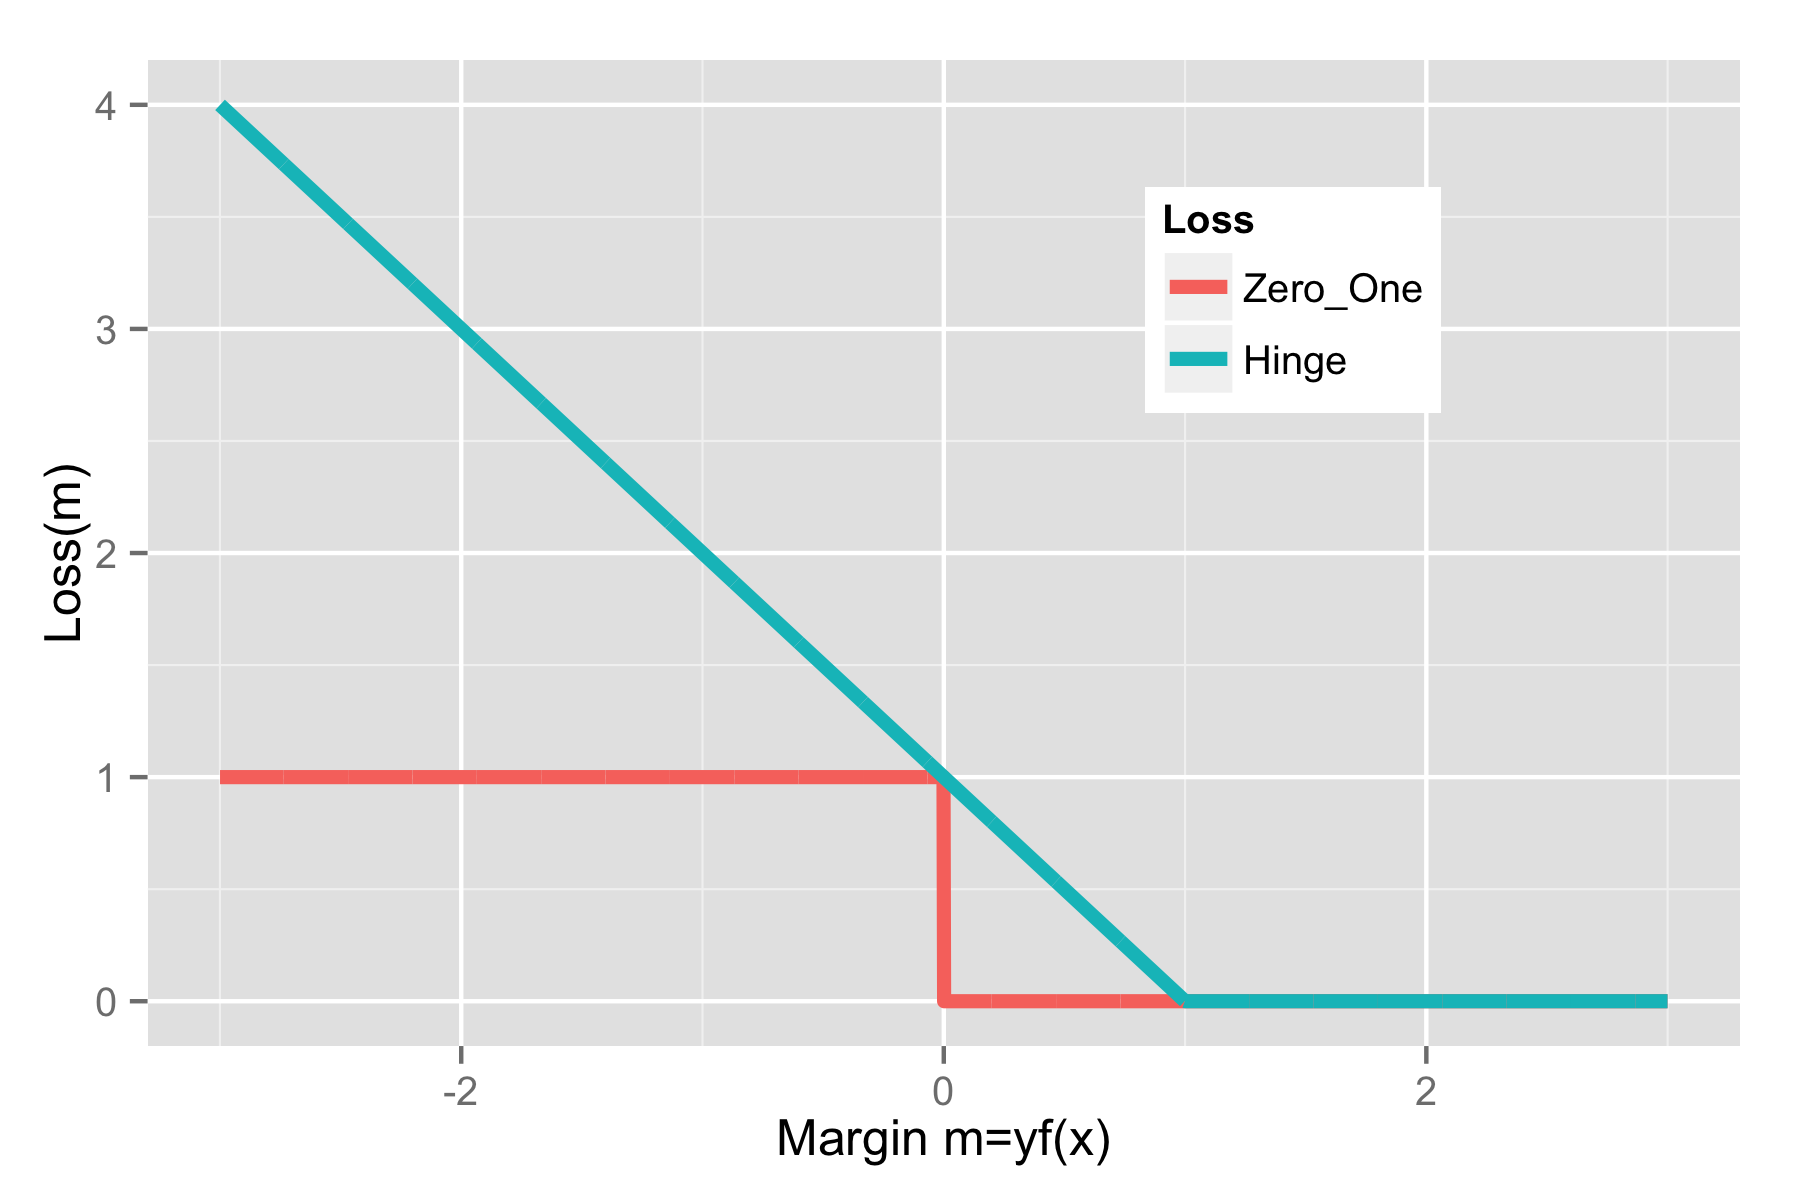
\includegraphics[height=4cm]{figures/loss.Zero_One.Hinge.png}
    \end{figure}
    \begin{itemize}
        \item A (sub)differentiable upperbound of the zero-one loss
        \item Not differentiable at $\text{margin}=1$ (use subgradients)
        %\item Subgradient: $\pc{g\colon f(x) \ge x_0 + g^T(x-x_0)}$
    \end{itemize}
\end{frame}

\begin{frame}
    {Logistic loss}
    $$
    L(x,y,f_w) = \log(1+e^{-yf_w(x)})
    $$
    \begin{figure}
        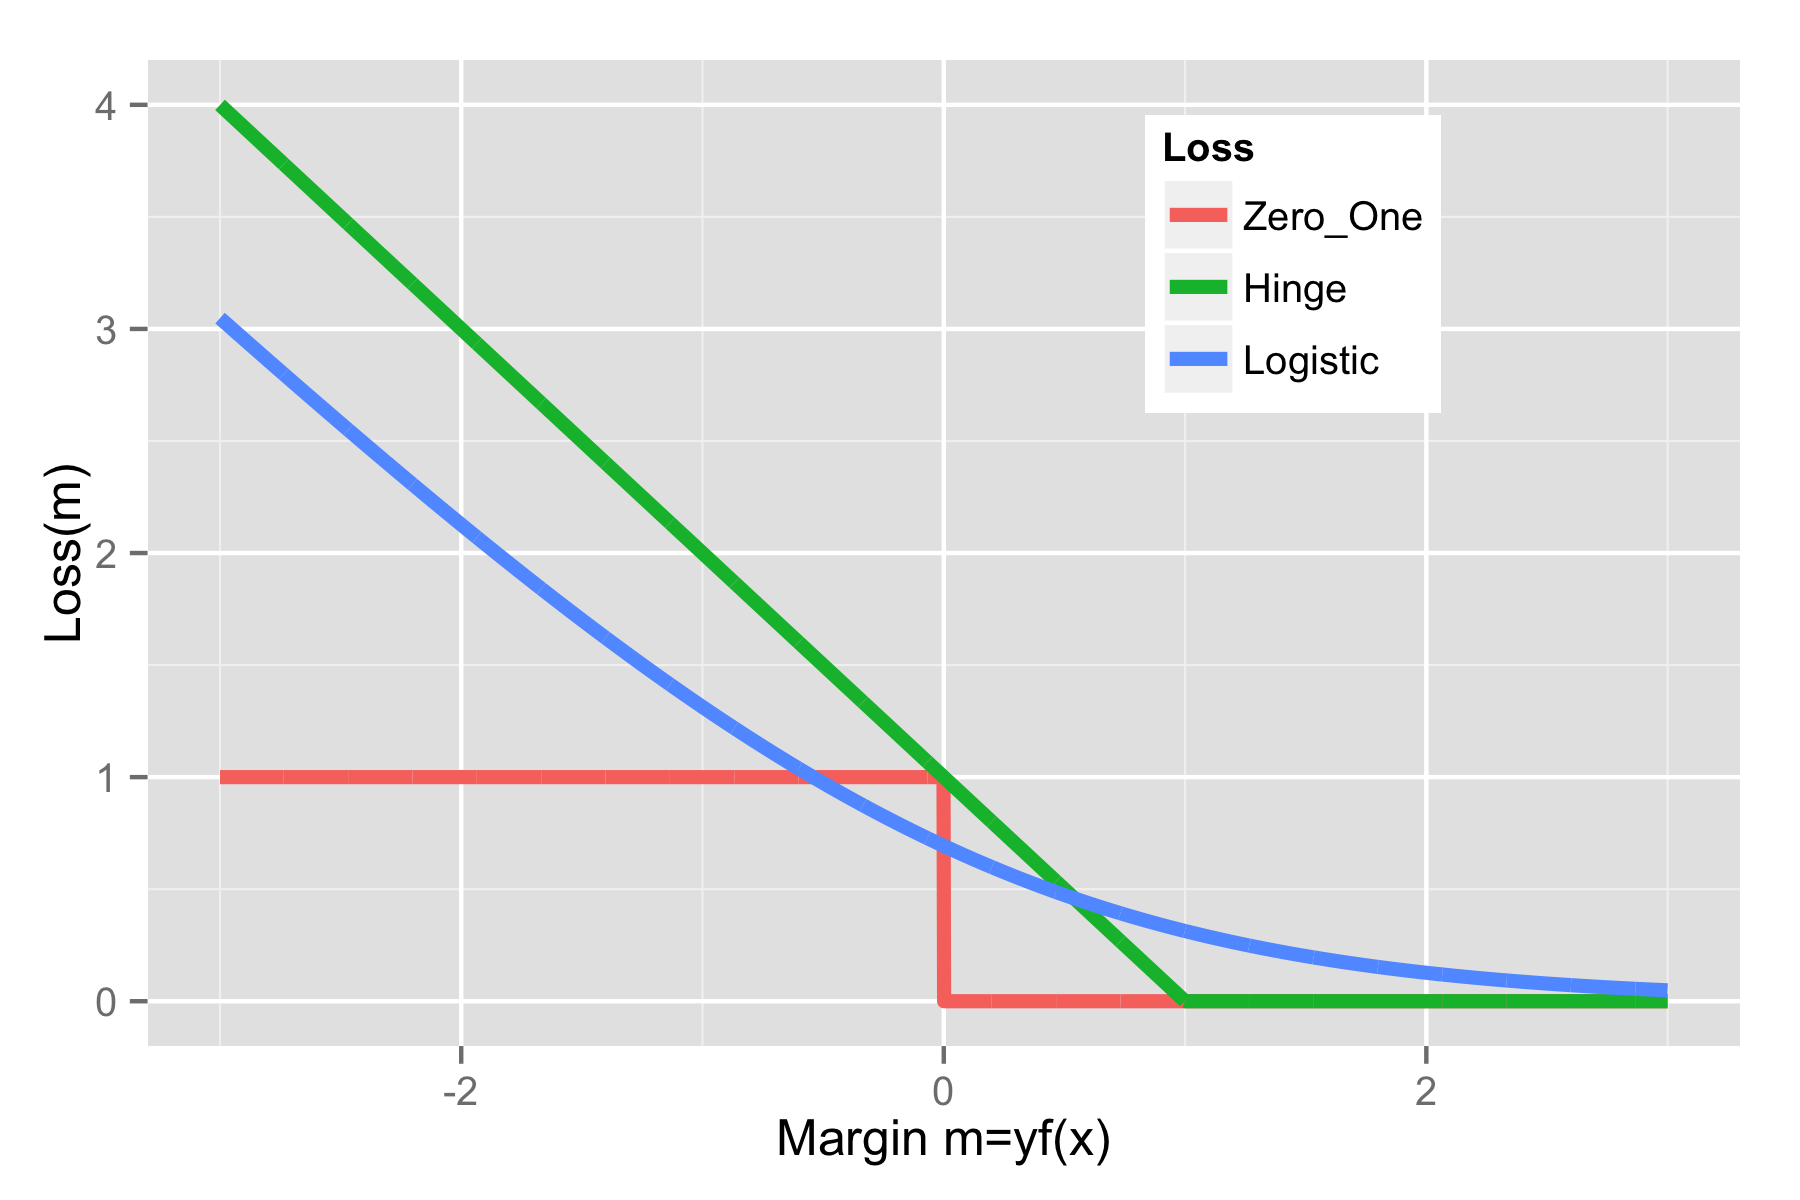
\includegraphics[height=4cm]{figures/loss.Zero_One.Hinge.Logistic.png}
    \end{figure}
    \begin{itemize}
        \item Differentiable
        \item Always wants more margin (loss is never 0)
    \end{itemize}
\end{frame}

\begin{frame}
    {Summary}
    \begin{enumerate}
        \itemsep2em
        \item Obtain training data $D_{\text{train}}=\pc{(x^{(i)}, y^{(i)})}_{i=1}^n$.
        \item Choose a loss function $L$ and a hypothesis class $\sH$ (\blue{domain knowledge}).
        \item Learn a predictor by minimizing the empirical risk (\blue{optimization}).
    \end{enumerate}
\end{frame}


\section{Optimization}

\begin{frame}
    {Gradient descent}
    \begin{itemize}
        \item The gradient of a function $F$ at a point $w \in \BR^d$ is the direction of fastest increase in the function value
        \item To minimze $F(w)$, move in the opposite direction
        $$w \leftarrow w - \eta\nabla_w F(w)$$
        \item Converge to a local minimum (also global minimum if $F(w)$ is \textbf{convex}) with carefully chosen step sizes $\eta$
    \end{itemize}
\end{frame}

\begin{frame}
    {Stochastic gradient descent}
    \begin{itemize}
        \item \textbf{Gradient descent (GD)} for ERM
            $$
            w \leftarrow w - \eta\nabla_w \underbrace{\sum_{i=1}^n L(x^{(i)}, y^{(i)}, w)}_{\textstyle{\text{training set loss}}}
            $$
            \pause
        \item \textbf{Stochastic gradient descent (SGD)}: take \blue{noisy but faster} updates\\
            \begin{align*}
                \text{For each } &(x, y) \in D_{\text{train}}:\\
                &w \leftarrow w - \eta\nabla_w \underbrace{L(x, y, f_w)}_{\textstyle{\text{example loss}}}
            \end{align*}
    \end{itemize}
\end{frame}

\begin{frame}
    {GD vs SGD}
    \begin{figure}
        \caption{Minimize $1.25(x + 6)^2 + (y - 8)^2$. Example from ``Understanding Machine Learning: From Theory to Algorithms''}
        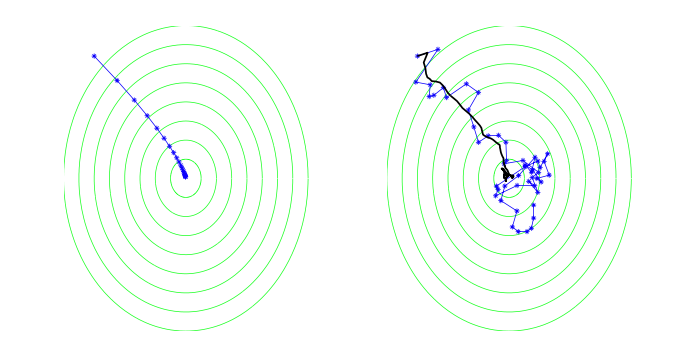
\includegraphics[height=5cm]{figures/gd-vs-sgd}
    \end{figure}
    SGD step is noisier as it gets closer to the optimum; need to reduce step size gradually.
\end{frame}

\begin{frame}
    {SGD summary}
    \begin{itemize}
        \itemsep1em
        \item Each update is efficient in both time and space
        \item Can be slow to converge 
        \item Popular in large-scale ML, including non-convex problems
        \item In practice, 
            \begin{itemize}
                \item Randomly sample examples.
                \item Fixed or diminishing step sizes, e.g. $1/t$, $1/\sqrt{t}$.
                \item Stop when objective does not improve.
            \end{itemize}
        \item Our main optimization techinque
    \end{itemize}
\end{frame}

\begin{frame}
    {Summary}
    \begin{itemize}
        \itemsep2em
        \item Choose hypothesis class based on domain knowledge
        \item Learning algorithm: empirical risk minimization
        \item Optimization: stochastic gradient descent
    \end{itemize}
\end{frame}

\end{document}
